%Chapter 3 outlines the Problem Formulation and Approach, including
%High level pipeline design of fully integrated system (from proposal with modification)
%Break down into sub-problems to be solved
\chapter{Problem and Approach}
\label{chap:approach}
Ultimately my goal is to create a software suite that will take RGB-D data from a Kinect or equivalent sensor and add the new information from each successive frame into a mesh-based representation of the world (ideally in real time). The target use case for the system is indoor environments. Human built environments tend to be dominated by planar surfaces, which if segmented out from the image can be processed and stored very efficiently. Since even planar segments with tattered edges require very few triangles to accurately represent them, the hope is that the majority of the scene can be stored with relatively few triangles.\par
To accomplish all of this in real time, most of the processing will be maintained on the GPU and host-device memory transfers will be minimized. Keeping the bulk of the pipeline on the GPU has many challenges. Existing algorithms have to be heavily modified or re-imagined to run optimally in a data parallel environment. To avoid costly synchronization delays, most of the pipeline must also be designed to accommodate anomalous data without CPU intervention or even acknowledgement. GPU architecture does not offer a simple way to return results from a kernel, so returning flags for success or failure is difficult to accomplish efficiently.\par

This thesis presents an implementation of a large portion of the planned pipeline. The pipeline segments out planar segments and converts them to textured meshes using a QuadTree based triangulation scheme.
\section{High Level System Design}
Figure~\ref{fig:toplevelpipeline} shows the planned pipeline at the highest level of organization. The haloed blocks represent the portions of the pipeline that are implemented in this thesis. The other blocks are provided for context, as some of the design features of this thesis would make little sense without the end goal in mind. For the remainder of this chapter I will describe the function of each module in Figure~\ref{fig:toplevelpipeline}. The specific implementation of each module will be explained in much greater detail in Chapter~\ref{chap:implementation}.


\begin{figure}[hp]
    \centering
    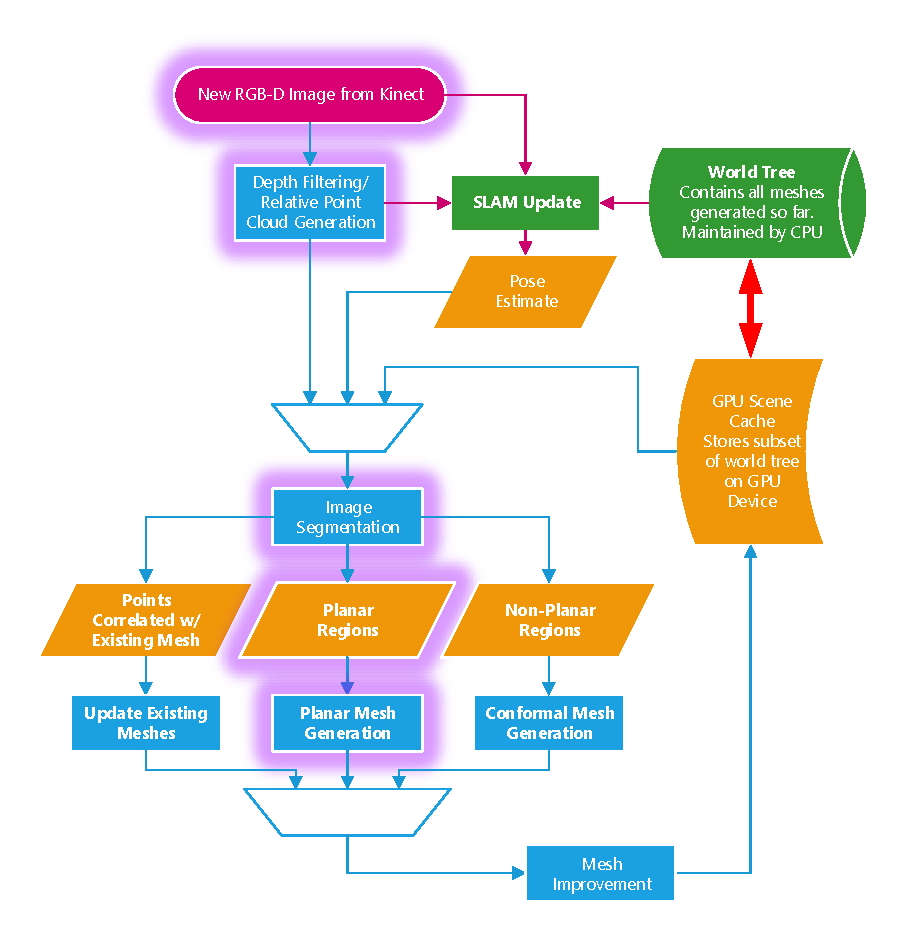
\includegraphics[width=1.0\textwidth]{TopLevelPipeline.pdf}
    \caption{Planned pipeline design. Highlighted blocks represent this thesis.}
    \label{fig:toplevelpipeline}
\end{figure}

\subsection{New RGB-D Image}
This thesis presents a custom open-source highly modular framework which allows the pipeline to take its RGB-D data from a variety of sources without knowing the implementation details. Currently the framework can only read from a Kinect via OpenNI or from a log generated by the logging tool I developed with the same framework. However, the modular nature of the code allows new data sources to be very easily incorporated.

\subsection{World Tree}
The world tree will be maintained in main computer memory by the CPU. It will store the complete mesh representation of the world in a hierarchical tree data structure similar to a scene graph. Unlike a generic scene graph, this structure will be maintained as a strict tree. Each leaf node will contain a single mesh object. Each mesh's component vertices will be stored in an object local reference frame. Objects will be transformed into world space through a series of transformations stored in each node of the tree. This system allows objects to be easily grouped for efficient rendering and simple manipulation.

\subsection{GPU World Cache}
To reduce data redundancy and GPU memory usage, the GPU will only have direct access to a device cached subset of the world tree. The optimal heuristics for maintaining the integrity and efficiency have not been developed yet, but the goal is to maintain a GPU copy of all known meshes in the Kinect's current field of view and those likely to come into view in the next few frames. The cache synchronization with the world tree and subset selection will be handled by the CPU.

\subsection{Input Processing and SLAM}
The raw RGB-D image from the kinect sensor is first passed to the GPU so the data can be filtered and processed in parallel. Once the data is processed, the SLAM algorithm will complete its pose estimation processing, combining the current world model as stored in the world tree and the 3D features from the newly generated point cloud.

\subsection{Image Segmentation}
Using a combination of information from the processed RGB-D frame, the current camera pose estimate, and the GPU cached world model, each point in the frame's point cloud will be segmented into three categories: points that correspond to parts of the existing mesh world, uncorrelated planar regions, and uncorrelated non-planar regions. Each category will be processed very differently at the next stage, so generating a robust segmentation will be crucial. Within each category, individual regions will be indexed so they can be easily processed in a region parallel manner for the meshing stage.\par
For this thesis, only planar regions are detected.

\subsection{Meshing}
Each region generated by the segmentation stage will be processed in parallel and in a very different way.
\subsubsection{Correlated Points}
Points determined to correspond to existing meshes will be used to update the existing meshes. Points will be used to add new vertices to a mesh as needed for added detail or to increase confidence in existing vertex estimates. This process allows the pipeline to take full advantage of higher resolution/closer capture frames of previously seen meshes. RGB data will also be used to update model texturing, allowing for texture quality improvement.

\subsubsection{Planar Regions}
Planar regions are projected to a best-fit true plane and triangulated using a QuadTree-Based (QTB) triangulation algorithm inspired by previous efforts\cite{planesegmentationQTB,ma2013planar}. The method has been demonstrated to efficiently decimate points clouds and dramatically simplifies triangulation and texture generations. In the future, if a planar region is determined to overlap with an existing plane, the existing quad-tree will be expanded to incorporate the new information.

\subsubsection{Non-planar Regions}
The remaining regions will be triangulated and converted into a new non-planar mesh object using simple polygon based triangulation method. Since conforming texture generation with arbitrary surfaces is a difficult problem to solve in real time with minimal distortion, non-planar meshes will be vertex colored. With a detailed enough triangulation, the visual quality of the of vertex shading is favorably comparable to a textured mesh. The framework would allow for simple addition of textures later if a texture would be a more efficient representation.

\subsection{Mesh Improvement}
Once individual mesh regions have been generated, meshes will be checked for easy optimizations and the potential for mesh merging. The goal of this stage is to reduce the number of vertices and distinct objects. This step is optional and not required for the pipeline to function, but it can help to simplify the representation and avoid unnecessarily fragmenting the world map. 
